\documentclass[sigplan,10pt]{acmart}

\AtBeginDocument{%
  \providecommand\BibTeX{{%
    \normalfont B\kern-0.5em{\scshape i\kern-0.25em b}\kern-0.8em\TeX}}}

\usepackage{xspace}
\usepackage[labelformat=simple]{subcaption}
\usepackage{tikz}
\usepackage{fancyvrb}
\usepackage{xcolor}
\usepackage{breqn}

\setcopyright{acmcopyright}
\copyrightyear{2020}
\acmYear{2020}
\acmDOI{10.1145/1122445.1122456}

%% These commands are for a PROCEEDINGS abstract or paper.
\acmConference[PaPoC '20]{PaPoC '20: Proceedings of the 7th Workshop on Principles and Practice of Consistency for Distributed Data}{April 27, 2020}{Heraklion, Crete, Greece}
\acmBooktitle{PaPoC '20: Proceedings of the 7th Workshop on Principles and Practice of Consistency for Distributed Data, April 27, 2020, Heraklion, Crete, Greece}
\acmPrice{15.00}
% \acmISBN{978-1-4503-XXXX-X/18/06}

% Submission ID.
% Use this when submitting an article to a sponsored event. You'll
% receive a unique submission ID from the organizers
% of the event, and this ID should be used as the parameter to this command.
%\acmSubmissionID{123-A56-BU3}

\begin{document}

\title{Preserving Reciprocal Consistency in Distributed Graph Databases}

\author{Jack Waudby}
\email{j.waudby2@ncl.ac.uk}
\affiliation{%
  \institution{Newcastle University}
  \city{Newcastle}
  \country{UK}
  \postcode{NE4 5TG}
}

\author{Paul Ezhilchelvan}
\email{paul.ezhilchelvan@ncl.ac.uk}
\orcid{0000-0002-6190-5685}
\affiliation{%
  \institution{Newcastle University}
  \city{Newcastle}
  \country{UK}
  \postcode{NE4 5TG}
}

\author{Jim Webber}
\email{jim.webber@neo4j.com}
\affiliation{%
  \institution{Neo4j}
  \streetaddress{Union House,182-194 Union Street}
  \city{London}
  \country{UK}
  \postcode{SE1 0LH}}

\author{Isi Mitrani}
\email{isi.mitrani@ncl.ac.uk}
\orcid{0000-0002-7797-7755}
\affiliation{%
  \institution{Newcastle University}
  \city{Newcastle}
  \country{UK}
  \postcode{NE4 5TG}
}

\renewcommand{\shortauthors}{Waudby, et al.}

\begin{abstract}
  Our earlier work identifies \emph{reciprocal consistency} as an important property that must be preserved in distributed graph databases.
  It also demonstrates that a failure to do so seriously undermines the integrity of the database itself in the long term.
  Reciprocal consistency can be maintained as a part of enforcing any known isolation guarantee and such an enforcement is also known to lead to reduction in performance. Therefore, in practice, distributed graph databases are often built atop BASE databases with no isolation guarantees, benefiting from good performance but leaving them susceptible to corruption due to violations of reciprocal consistency.
  This paper designs and presents a lightweight, locking-free protocol and then evaluates the protocol's abilities to preserve reciprocal consistency and also offer good throughput. Our evaluations establish that  the protocol can offer both integrity guarantees and sound performance when the value of its parameter is chosen appropriately.
\end{abstract}

% \begin{CCSXML}
% <ccs2012>
%  <concept>
%   <concept_id>10010520.10010553.10010562</concept_id>
%   <concept_desc>Computer systems organization~Embedded systems</concept_desc>
%   <concept_significance>500</concept_significance>
%  </concept>
%  <concept>
%   <concept_id>10010520.10010575.10010755</concept_id>
%   <concept_desc>Computer systems organization~Redundancy</concept_desc>
%   <concept_significance>300</concept_significance>
%  </concept>
%  <concept>
%   <concept_id>10010520.10010553.10010554</concept_id>
%   <concept_desc>Computer systems organization~Robotics</concept_desc>
%   <concept_significance>100</concept_significance>
%  </concept>
%  <concept>
%   <concept_id>10003033.10003083.10003095</concept_id>
%   <concept_desc>Networks~Network reliability</concept_desc>
%   <concept_significance>100</concept_significance>
%  </concept>
% </ccs2012>
% \end{CCSXML}

\ccsdesc[500]{Data Management~Graph Databases}
\ccsdesc[300]{Data Management~Reciprocal Consistency}
\ccsdesc[300]{Data Management~Concurrency Control}

\keywords{Graph Databases, Reciprocal Consistency, BASE}

\maketitle

\section{Introduction}
\label{sec:introduction}

Recent years have seen a proliferation in the use of graph processing technologies \cite{Besta2019}. Application areas are wide reaching from healthcare, to social networks and fraud detection \cite{Eifrem2016}. Graph databases model data as a \textit{property graph} \cite{Robinson2015}, vertices represent entities and edges represent the relationships between entities. In addition, properties can be stored on both vertices and edges. In the storage layer, edges are represented by two reciprocal pointers, one stored with each vertex the edge connects. This allows for bi-directional traversal and improved query performance \cite{Robinson2015}. An edge is said to be \emph{reciprocally consistent}, if its two end pointers are mutually reciprocal of each other (details in Section \ref{sec:recipr-cons}).

In practice, graphs can be extremely large, sometimes in the magnitude of 100 billion edges \cite{Sahu2017}, exceeding the storage capacity of a single-node graph database and motivating the need for distributed graph databases. A common distributed graph database design pattern is to first partition graph data over several machines in a cluster; resulting in a number of \emph{distributed edges}, an edge's reciprocal pointers reside in different partitions. Recent work \cite{Ezhilchelvan2018} and \cite{Webber2019} highlighted that violations of reciprocal consistency in distributed edges introduce corruption into the database. Moreover, due to the \emph{Scale-Free} \cite{ScaleFree} property exhibited by many real world graphs, this corruption can propagate through the database at alarmingly rates.

When, for example, a BASE database \cite{Pritchett2008} is adapted with a graph processing layer, then violations of reciprocal consistency will occur if that adaptation provides no concurrency control for operations that span partitions in order to offer higher performance. This paper proposes a simple concurrency control protocol, called \tDelta protocol, that does not impede performance adversely. That is because the protocol is exclusively designed for one purpose only: reciprocal consistency in distributed edges.  Its design leverages the fact that the updating of end pointers of a given distributed edge immediately follow each other and the small interval between them is the window for possible conflicts between concurrent updates.

The paper is organized as follows: Section \ref{sec:recipr-cons} presents reciprocal consistency, Sections \ref{sec:distr-graph-datab}-\ref{sec:db-corruption} discuss the architecture of distributed graph databases and describes how corruption occurs. Section \ref{sec:tdelta-protocol} outlines the \tDelta protocol. Sections \ref{sec:modeling}-\ref{sec:evaluation} presents the model used to evaluate protocol performance.


\section{Reciprocal Consistency}
\label{sec:recipr-cons}

In the property graph data model edges have direction, each edge having a pair of \emph{source} and \emph{destination} vertices.
In the storage layer, edge information is stored with \textbf{both} the source and destination vertices.
This, as we explain next, allows an edge to be traversed in both directions and thus facilitates improved query performance.

A common approach to storing graphs (arising from JanusGraph \cite{janusgraph} and TitanDB \cite{TitanDB}) is given in Figure \ref{adj-list}.
A vertex is represented by a record that contains one or more vertex properties and a sequence of edge pointers (each shown simply as edge in Figure \ref{adj-list}) pointing to other vertices.
This sequence of edge pointers is referred to as an adjacency list.

Consider, for example, the statement that Tolkien \textit{wrote} The Hobbit.
It is expressed using vertices \emph{a} and \emph{b}, for Tolkien and The Hobbit respectively, and an edge \textit{wrote} running from \emph{a} (source) to \emph{b} (destination).

Using openCypher \cite{openCypher} this can be represented by:
\begin{Verbatim}[commandchars=\\\{\},fontsize=\small,xleftmargin=.2in]
\textcolor{blue}{MATCH} (a:\textcolor{green}{Person}), (b:\textcolor{green}{Book})
\textcolor{blue}{WHERE} a.\textcolor{red}{name} = 'Tolkien' \textcolor{blue}{AND} b.\textcolor{red}{title} = 'The Hobbit'
\textcolor{blue}{CREATE} (a)-[w:\textcolor{green}{WROTE}]->(b)
\end{Verbatim}

Adjacency lists of both \emph{a} and \emph{b} record information about the edge and this information is reciprocal (or inverse) of each other: \emph{a}'s list will indicate `\emph{a} \emph{wrote} \emph{b}' while \emph{b}'s will have `\emph{b} \emph{written} by \emph{a}', Figure \ref{reciprocally-consistent-edge}. Thus, a query `list all titles by the author who wrote The Hobbit' can be answered starting at (destination vertex) \emph{b} and then traversing to (source vertex) \emph{a}, even though the edge is ``directed'' from \emph{a} to \emph{b} at model level abstraction. When the adjacency list entries for a given edge are mutually compatible like this, that edge is said to be \emph{reciprocally consistent}, a form of referential integrity. A query can read either the source or destination vertex and is able to reify the edge correctly, returning consistent results.

\begin{figure}[ht!]
  \centering
  \begin{tikzpicture}[node distance=2cm]
    \node (v1) [big_vertex,xshift=0cm,yshift=0cm] {\small{\texttt{a:\textcolor{green}{Person}}}};

    \node (v2) [big_vertex,xshift=5cm,yshift=0cm] {\small{\texttt{b:\textcolor{green}{Book}}}};

    \node [below of=v1,yshift=1cm] {\small{\texttt{\textcolor{red}{name}:Tolkien}}};
        \node [below of=v2,yshift=1cm] {\small{\texttt{\textcolor{red}{title}:The Hobbit}}};

    \draw [thick,->,>=stealth] (0.8,0)  -- node [midway,above] {:\textcolor{green}{\small{\texttt{WROTE}}}} (4.2,0);
  \end{tikzpicture}
  \caption{A reciprocally consistent edge.}
  \label{reciprocally-consistent-edge}
\end{figure}

\section{Distributed Graph Databases}
\label{sec:distr-graph-datab}

A distributed graph database employs a shared-nothing architecture, partitioning a graph between a number of loosely cooperating servers.
Graph partitioning is non-trivial and a common approach is to use a $k$-balanced edge cut \cite{Huang2016}.
The objective of such an approach is to minimize the proportion of edges that span partitions in a manner that balances the distribution of vertices to partitions.
Figure \ref{dist-graph} depicts a graph database partitioned across 3 servers, $S1$, $S2$ and $S3$.
Intra-partition edges are referred to as \textit{local edges} and inter-partition edges are referred to as \textit{distributed edges} (shown with dashed lines in Figure \ref{dist-graph}).
The proportion of distributed edges is always non-negligible ranging from 25-75\% \cite{Huang2016}.

\begin{figure}[ht]
  \centering
    \begin{tikzpicture}[node distance=1cm]

    \node (s1) [server,label=$S_1$] {};
    \node (s2) [server, right of=s1,xshift=1.5cm,yshift=1cm,label=$S_2$] {};
    \node (s3) [server, right of=s1,xshift=4cm,label=$S_3$] {};

    \node (v1) [vertex,xshift=-0.5cm,yshift=-0.8cm] {};
    \node (v2) [vertex, above of=v1,xshift=-0.1cm,yshift=0.7cm] {};
    \node (v3) [vertex, above of=v1,xshift=0.6cm] {};
    \node (v4) [vertex, below right of=v3,xshift=-0.5cm,yshift=-0.25cm] {};
    \node (v5) [vertex, above right of=v3,xshift=-0.1cm,yshift=-0.2cm] {};
    \node (v6) [vertex, right of=v5,xshift=0.5cm,yshift=0.8cm] {};
    \node (v7) [vertex, below of=v6, xshift=-0.15cm,yshift=0cm] {};
    \node (v8) [vertex, right of=v4, yshift=-0.1cm,xshift=4cm] {};
    \node (v9) [vertex, above of=v8,xshift=-0.4cm,yshift=-0.5cm] {};
    \node (v10) [vertex, above of=v9,xshift=-1.7cm,yshift=-0.33cm] {};
    \node (v11) [vertex, right of=v9,yshift=0.5cm,xshift=-0.3cm] {};
    \node (v12) [vertex, above of=v11,yshift=-0.3cm,xshift=-1cm] {};
    \node (v13) [vertex, above right of=v6,yshift=-0.4cm,xshift=-0.1cm] {};
    \draw [local] (v2) -- (v1);
    \draw [local] (v1) -- (v3);
    \draw [local] (v3) -- (v2);
    \draw [local] (v2) -- (v5);
    \draw [local] (v1) -- (v4);
    \draw [local] (v5) -- (v4);
    \draw [dist] (v5) -- (v6);
    \draw [dist] (v4) -- (v7);
    \draw [dist] (v8) -- (v4);
    \draw [local] (v8) -- (v9);
    \draw [local] (v9) -- (v11);
    \draw [local] (v10) -- (v7);
    \draw [dist] (v10) -- (v12);
    \draw [dist] (v12) -- (v13);
    \draw [local] (v10) -- (v6);
    \draw [dist] (v10) -- (v11);
    \draw [local] (v13) -- (v10);
    \draw [local] (v11) -- (v12);
    \end{tikzpicture}
  \caption{Local and distributed edges}
  \Description{Graph representation.}
  \label{dist-graph}
\end{figure}


Adjacency lists can now contain edge pointers to vertices on remote servers. Maintaining reciprocal consistency for distributed edges is challenging - especially given an architecture employed by contemporary distributed graph databases (\cite{janusgraph}, \cite{TitanDB}). Often an existing BASE database is used for storage, which is then adapted with a query language expressed in terms of edges and vertices along with some gluecode to bind that interface to the underlying database - we refer to such systems as BASE distributed graph databases\footnote{Typically, each partition is replicated for fault tolerance and availability, these issues are beyond the scope of this paper.}. Superficially, opting for this design appears to be a good choice: the application programmer has the modeling convenience of graphs with the operational characteristics from the underlying BASE database.

However, the problem with this design is the (lack of) transactional semantics is inherited from the underlying database. BASE databases seldom provide guarantees for multi-operation, multi-object transactions that span partitions. This lack of concurrency control across partitions makes it possible for concurrent updates to interleave in a manner that violates reciprocal consistency of distributed edges\footnote{When operating without concurrency control it is equally possible that local edges become reciprocal consistent, however primitives provided by BASE databases are typically sufficient to ensure reciprocal consistency for local edges.}. Earlier work investigated how the lack of concurrency control across partitions can undermine reciprocal consistency of distributed edges, causing irreversible corruption that spreads at alarmingly rates (\cite{Ezhilchelvan2018}, \cite{Webber2019}). This process is explained in Section \ref{sec:db-corruption}.

\begin{figure*}[ht]
  \centering
  \begin{subfigure}[b]{0.3\textwidth}
    \centering
    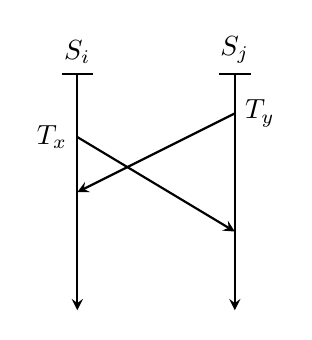
\begin{tikzpicture}
      \draw [thick] (1.3,3) -- (1.7,3);
      \draw [thick,<-,>=stealth] (1.5,0) -- (1.5,3) node[anchor=south] {$S_i$};
      \draw [thick] (3.3,3) -- (3.7,3);
      \draw [thick,<-,>=stealth] (3.5,0) -- (3.5,3) node[anchor=south] {$S_j$};
      \draw [thick,<-,>=stealth] (1.5,1.5) -- (3.5,2.5)  node[right] {$T_y$};
      \draw [thick,->,>=stealth] (1.5,2.2) node[left] {$T_x$} -- (3.5,1);
    \end{tikzpicture}
    \caption{}
    \label{fig:tx-ty}
  \end{subfigure}%
  \begin{subfigure}[b]{0.3\textwidth}
    \centering
    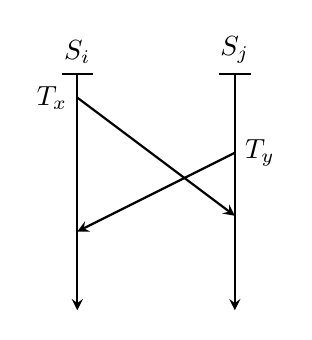
\begin{tikzpicture}
      \draw [thick] (5.3,3) -- (5.7,3);
      \draw [thick,<-,>=stealth] (5.5,0) -- (5.5,3) node[anchor=south] {$S_i$};
      \draw [thick] (7.3,3) -- (7.7,3);
      \draw [thick,<-,>=stealth] (7.5,0) -- (7.5,3) node[anchor=south] {$S_j$};
      \draw [thick,<-,>=stealth] (5.5,1) -- (7.5,2)  node[right] {$T_y$};
      \draw [thick,->,>=stealth] (5.5,2.7) node[left] {$T_x$} -- (7.5,1.2);
    \end{tikzpicture}
    \caption{}
\label{fig:ty-tx}
  \end{subfigure}%
  \begin{subfigure}[b]{0.3\textwidth}
    \centering
    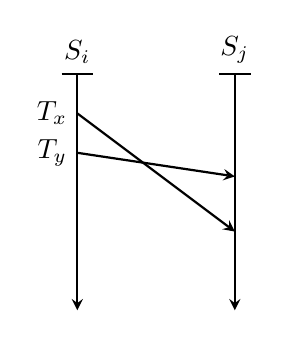
\begin{tikzpicture}
      \draw [thick] (9.3,3) -- (9.7,3);
      \draw [thick,<-,>=stealth] (9.5,0) -- (9.5,3) node[anchor=south] {$S_i$};
      \draw [thick] (11.3,3) -- (11.7,3);
      \draw [thick,<-,>=stealth] (11.5,0) -- (11.5,3) node[anchor=south] {$S_j$};
      \draw [thick,->,>=stealth] (9.5,2.5)  node[left] {$T_x$} -- (11.5,1) ;
      \draw [thick,->,>=stealth] (9.5,2) node[left] {$T_y$} -- (11.5,1.7);
    \end{tikzpicture}
    \caption{}
    \label{fig:same-side}
  \end{subfigure}%
  \caption{Possible interleavings of concurrent transaction's writes to a distributed edge spanning servers $S_i$ and $S_j$ by transactions $T_x$ and $T_y$. In \subref{fig:tx-ty} $T_y$ begins writing to the distributed edge before $T_x$, in \subref{fig:ty-tx} the converse is true, else they are equivalent. In \subref{fig:same-side} both transactions begin writing at the same server but overlap in the network and arrive out-of-order.}
  \label{conf-scen}
\end{figure*}


\section{Corruption in the Absence of Concurrency Control}
\label{sec:db-corruption}

When a given transaction writes a distributed edge it must infact perform two writes, writing reciprocal entries in the adjacency lists at the source and the destination vertices, which say reside on servers $S_i$ and $S_j$ respectively. Without concurrency control, transaction's writes to a distributed edge can interleave producing a distributed edge in a \emph{half-corrupted} state - reciprocal consistency has been violated. Possible interleavings of concurrent writes to a distributed edge are given in Figure \ref{conf-scen}. A half-corrupted edge is an example of a \emph{dirty write} (ANSI \emph{P0} \cite{Berenson1995}, Adya \emph{G0} \cite{Adya2000}), which is proscribed by the weakest ANSI isolation level \textbf{Read Uncommitted}. Under Read Uncommitted the database ensures a total order on transactions, consistently ordering writes from concurrent transactions, which would prevent all interleavings in Figure \ref{conf-scen}.

For such half-corrupted edges there exists a correct and a incorrect entry. Note, the order in which the two writes take place is not constrained. For example, when updating an edge between \emph{a} and \emph{b} it is equally likely to update \emph{a} then \emph{b} as it is to update \emph{b} then \emph{a}. A graph with half-corrupted edges has suffered \emph{structural corruption}.

Now, if subsequent transactions read the incorrect entry of a half-corrupted edge and write further edges, \emph{semantic corruption} has been introduced into the database. Further semantic corruption spreads by the same mechanism. A database is said to be \emph{operationally corrupt} when a significant proportion of its data records are in a semantically corrupted state, rendering the database of little practical use. To illustrate the process of corruption, consider two transactions $T_x$ and $T_y$. $T_x$ deletes the \emph{wrote} edge and $T_y$ appends a property \emph{year}:
\begin{Verbatim}[commandchars=\\\{\},fontsize=\small,xleftmargin=.2in]
\textcolor{grey}{// Tx}
\textcolor{blue}{MATCH} (a:\textcolor{green}{Person})-[w:\textcolor{green}{WROTE}]->(b:\textcolor{green}{Book})
\textcolor{blue}{WHERE} a.\textcolor{red}{name} = 'Tolkien' \textcolor{blue}{AND} b.\textcolor{red}{title} = 'The Hobbit'
\textcolor{blue}{DELETE} w

\textcolor{grey}{// Ty}
\textcolor{blue}{MATCH} (a:\textcolor{green}{Person})-[w:\textcolor{green}{WROTE}]->(b:\textcolor{green}{Book})
\textcolor{blue}{WHERE} a.\textcolor{red}{name} = 'Tolkien' \textcolor{blue}{AND} b.\textcolor{red}{title} = 'The Hobbit'
\textcolor{blue}{SET} w.\textcolor{red}{year} = 1937
\end{Verbatim}
Any interleaving in Figure \ref{conf-scen} will result in the half-corrupted edge displayed in Figure \ref{half-corrupted}. Assume, the correct ordering of transactions is $T_y$ then $T_x$ and the edge between \emph{a} and \emph{b} should still exist. The following transaction, $T_z$, introduces semantic corruption if it starts at \emph{b} and adds a new \emph{wrote} edge to an ``unknown author'' vertex. Further corruption spreads by the same mechanism.

\begin{Verbatim}[commandchars=\\\{\},fontsize=\small,xleftmargin=.2in]
\textcolor{grey}{// Tz}
\textcolor{blue}{MATCH} (b:\textcolor{green}{Book}),(u:Person)
\textcolor{blue}{WHERE NOT} (:\textcolor{green}{Person})-[:\textcolor{green}{WROTE}]->(b:\textcolor{green}{Book})
\textcolor{blue}{AND} u.\textcolor{red}{name} = 'unknown'
\textcolor{blue}{CREATE} (u)-[:\textcolor{green}{WROTE}]->(b)
\end{Verbatim}


\section{\tDelta Protocol}
\label{sec:tdelta-protocol}

A straightforward solution to preventing dirty writes is for transactions to take long duration write locks \cite{Berenson1995}, releasing them only once the acquiring transaction has committed or aborted. To prevent deadlock a policy such as \texttt{NO_WAIT} deadlock detection is used, which was shown to be the optimal policy in a distributed, partitioned database \cite{Harding2017}.

Our \tDelta protocol employs principles behind all these well-tested strategies but has two crucial differences:
\begin{itemize}
\item No locks are used.
\item A write operation need not await until the preceding write commits but can proceed if at least $\Delta$ duration (measured in local clock) has elapsed.
\end{itemize}

These differences lead to several advantages in the context of graph databases. Firstly, a subset of edges are traversed and modified with a high frequency e.g. critical sections of motorway in a road network, leading to high contention. Secondly, graph transactions tend to be longer-lived than transactions in relational databases. Waiting for earlier writes on edges by long running transactions to commit, these frequently accessed edges significantly limit concurrency and reduce throughput. With these concerns in mind we developed the \tDelta protocol, which aimed at preventing edges becoming half-corrupted and hence quashing the seed of corruption whilst keeping performance at an acceptable level.\footnote{The \tDelta protocol is solely a concurrency control mechanism for distributed edges, guarantees about vertices, local edges are beyond the scope of this paper.}

\subsection{Protocol Description}
\label{sec:protocol-description}

The \tDelta Protocol has five rules:
\begin{enumerate}
\item A transaction's update on an end pointer of an edge is initially tentative which would become permanent only if that transaction is permitted to commit.
\item A tentative write is possible if the end pointer is either in a permanent state or the immediately preceding tentative update was done at least $\Delta$ time before (where time is measured as per local clock).
\item If a transaction successfully performs all its tentative updates, then it is permitted to commit; otherwise, it must abort.
\item A transaction commits, when all its tentative updates are made permanent, e.g., using an atomic commitment protocol.
\item Tentative updates of an aborting transactions are ignored. An ignored tentative update can make a new transaction abort for up to $\Delta$ time after it was created; it is harmless thereafter and can be garbage collected at any time.
\end{enumerate}

\subsection{Correctness Reasoning}
\label{sec:corr-reas}

Let us define $\delta$ as the bound estimate on the interval that may elapse between a transaction updating one end of a distributed edge at one server and updating the other end of the same edge at another server.

Let $\Delta$ be chosen such that $\Delta > \delta$. Now consider the interleaving in Figure \ref{fig:tx-ty} and let $t_x$ be the (global) time when $T_x$ starts at server $S_i$; similarly $t_y$ be the time $T_y$ starts at server $S_j$. Note $t_y < t_x$, i.e. $(t_x - t_y) > 0$.

Say, $T_y$ reaches $S_i$ at time $t_y + d$, where $d$ is the actual time elapsed between completing a tentative write at one end and starting at another end, let us assume that $d \leq \delta$. When $T_y$ arrives at $S_i$ it will find a tentative write done at time $t_x$. In this case, $t_y + d - t_x = d - (t_x-t_y) < d \leq \delta < \Delta$; so, $T_y$ will abort, preventing writes from interleaving and half-corrupting the edge. A similar arguments can be made for the scenario in with Figure \ref{fig:ty-tx}. For the interleaving in Figure \ref{fig:same-side}, if $t_y - t_x > \Delta$, then $T_y$ cannot overtake $T_x$ at $S_j$.

Assume that $d > \Delta$, i.e., the estimate $\delta$ does not hold at this moment. In Figure \ref{fig:tx-ty} interfering updates are avoided only if $t_y + d - t_x = d - (t_x-t_y) < d \leq \delta < \Delta$ otherwise, an edge becomes half-corrupted. This holds for the interleaving in \ref{fig:ty-tx}. Thus, in the extreme case $t_x = t_y$, reciprocal consistency is not guaranteed if $d > \Delta$ when the former exceeds its upper bound estimate $\delta$. For Figure \ref{fig:same-side}, if $d$ for $T_x$ is larger than $\Delta$, reciprocal consistency can be violated.

This protocol is strictly weaker than Read Uncommitted isolation, ensuring only writes to distributed edge are totally ordered, preserving reciprocal consistency. The benefit of this approach is reduced contention on frequently accessed distributed edges, as the time a transaction has exclusive access to a given distributed edge is decreased.

In summary, the \tDelta protocol attempts to prevent the occurrence of half-corrupted distributed edges by aborting transactions but if $\Delta$ is exceeded edge can become half-corrupted and process of corruption described in Section \ref{sec:db-corruption} can still occur. Two questions naturally arise regards the performance of the protocol. For different values of $\Delta$:
\begin{itemize}
\item Given distributed edges can still become half-corrupted if $\Delta$ is exceeded, by how much time does the protocol increase the time until operational corruption?
\item How many transactions are aborted as a result of the protocol?
\end{itemize}


%The two paragraphs (The protocol leverages... edge is lost) can be commented out.

%Figures 5 and 6 can be removed.

% The protocol leverages the fact that a transaction that writes at one end of a distributed edge, must then immediately write the other end. It is then assumed that the network delay between two servers can be predicted to be some $\Delta$. All writes are temporary and assumed to be made permanent by a later atomic commitment protocol once the transaction has completed. From this, a distributed edge write is allowed to proceed provided there is no other temporary write preceding it within $\Delta$; measured as per the local clock time. Figure \ref{delta-abort} shows an instance of the protocol preventing the interleaving in Figure \ref{conf-scen} (c), $T_x$ overtakes $T_y$ but is aborted when arriving at $S_j$ as $T_y$ has already wrote tentatively within $\Delta$. An aborted transaction, aborts any and every previous tentative write that it may have successfully completed. This protocol avoids all conflict scenarios in Figure \ref{conf-scen} provided $\Delta$ is not exceeded.



% \begin{figure}[H]
%   \centering
%   \begin{tikzpicture}[node distance=2cm]
%     % s1
%     \draw [thick] (1.3,3) -- (1.7,3);
%     \draw [thick,<-,>=stealth] (1.5,0) -- (1.5,3) node[anchor=south] {$S_i$};
%     % s2
%     \draw [thick] (3.3,3) -- (3.7,3);
%     \draw [thick,<-,>=stealth] (3.5,0) -- (3.5,3) node[anchor=south] {$S_j$};

%     \draw [thick,->,>=stealth] (1.5,2.5) node[left] {$T_x$} -- (3.5,0.5);
%     \draw [thick,->,>=stealth] (1.5,2) node[left] {$T_y$} -- (3.5,1.8);

%     \draw [thick,<->,>=stealth] (3.7,0.5) -- (3.7,1.8) node[midway,right] {$< \Delta$};

%   \end{tikzpicture}
%   \caption{An example of the \tDelta protocol preserving reciprocal consistency.}
%   \label{delta-abort}
% \end{figure}

% Correctly choosing $\Delta$ is paramount, as if it is exceeded all three conflict scenarios can still occur, resulting in half-corrupted edges and the spread of semantic corruption. Figure \ref{corruption-again} displays an example when the \tDelta protocol fails to maintain reciprocal consistency. The network delay between $S_i$ and $S_j$ is sufficiently large the total ordering of writes to the distributed edge is lost.

% \begin{figure}[H]
%   \centering
%   \begin{tikzpicture}[node distance=2cm]
%     \draw [thick] (1.3,3) -- (1.7,3);
%     \draw [thick,<-,>=stealth] (1.5,0) -- (1.5,3) node[anchor=south] {$S_i$};
%     \draw [thick] (3.3,3) -- (3.7,3);
%     \draw [thick,<-,>=stealth] (3.5,0) -- (3.5,3) node[anchor=south] {$S_j$};
%         \draw [thick,->,>=stealth] (1.5,2.7) node[left] {$T_x$} -- (3.5,0.8);
%     \draw [thick,<-,>=stealth] (1.5,1) -- (3.5,2.2)  node[right] {$T_y$};

%     \draw [thick,<->,>=stealth] (4.2,1) -- (4.2,2.2) node[midway,left] {$> \Delta$};
%     \draw [thick,<->,>=stealth] (0.8,1) -- (0.8,2.5) node[midway,right] {$> \Delta$};
%   \end{tikzpicture}
%   \caption{An example of the \tDelta protocol failing to preserve reciprocal consistency.}
%   \label{corruption-again}
% \end{figure}


\section{Modeling}
\label{sec:modeling}

To assess the protocols impact on time to operational corruption the model developed in \cite{Ezhilchelvan2018} was extended\footnote{An implementation and empirical evaluation in an existing systems was not performed as such an evaluation would have been impractical (need to compare database state at end of experiment with the linearizable truth), slow (real time) and expensive (requiring many hours of storage and compute time)}. A summary of the model is now provided, before discussing the extensions.

The system processes transactions that arrive in a Poisson stream with rate $\lambda$ per second. To simplify the model, each transaction contains a random number of read operations, $K$, followed by a single write. To model a scale-free graph, edges in the database are divided into $T$ types, popular edges types have higher access probabilities but are a smaller proportion of the total number of edges, $N$. For each type, a fraction $f$ are distributed edges and the remainder are local edges. The network delay between servers was assumed to be exponentially distributed with rate $\rho$. At any moment in time an edge can be in one of four states:
\begin{enumerate}
\item Local and clean.
\item Distributed and clean.
\item Half-corrupted distributed edge arising from a dirty write.
\item Semantically corrupted.
\end{enumerate}
% The valid state transitions are given in Figure \ref{state-transitions}. Note, only distributed edges can be in state 2, but any edge, including local ones, can be in state 3.

% \begin{figure}[ht]
%   \centering
%     \begin{tikzpicture}[node distance=2cm]
%       \node (n0) [circle,draw,radius=0.3, align=center,green] {0};
%       \node (n1) [circle,draw,radius=0.3, align=center, right of=n0,green] {1};
%       \node (n2) [circle,draw,radius=0.3, align=center, right of=n1,orange] {2};
%       \node (n3) [circle,draw,radius=0.3, align=center, right of=n2,red] {3};
%       \draw [thick,<-,>=stealth,green] (n1) to[out=-45,in=-135]  node[below] {$a_{2,1}$} (n2);
%       \draw [thick,->,>=stealth,orange] (n1)  to[out=0,in=-180] node[below] {$a_{1,2}$} (n2);
%       \draw  [thick,->,>=stealth,red] (n2) to[out=-45,in=-135]  node[below] {$a_{2,3}$} (n3);
%       \draw  [thick,->,>=stealth,red]  (n0) to[out=70,in=110] node[above] {$a_{0,3}$} (n3);
%       \draw  [thick,->,>=stealth,red]  (n1) to[out=45,in=135] node[above] {$a_{1,3}$} (n3);
%     \end{tikzpicture}
%     \caption{Edge transitions between clean, half-corrupted and semantically corrupt states.}
%     \label{state-transitions}
% \end{figure}

Probabilities are then derived for a given read operation returning a correct answer (states 1, 2 or the correct record in state 3) and all the reads by a given transaction returning correct answers. Then the probability of edge becoming half-corrupted $q_i$, by a given transaction arriving at time $t$ and operating on edge of type $i$ is derived. These probabilities are used to construct transition rates $a_{i,j}$ between states, which are used to simulate the process of corrupting the database and obtain estimates for the time to operational corruption, $U_{\gamma}$. At time $0$, all edges are clean (free from corruption), when a certain fraction, $\gamma$, of all edges become semantically corrupted, the database itself is said to be operationally corrupt. The reader is directed to \cite{Ezhilchelvan2018} and \cite{Webber2019} for a granular discussion of the initial model.

% (Appendix A)\footnote{To simplify the derivation of the new conflict probability it was assumed that messages sent from the same servers do not arrive out of order i.e. the interleaving in Figure 3(c) cannot occur.}.

The \tDelta protocol impacts the rate of corruption by reducing the probability a transaction corrupts a distributed edge, $q^{new}_i$. Of interest, therefore, is: how large or small is the value of $U_\gamma$ for a given value of $\gamma$ under the \tDelta protocol? Moreover, to quantify the number of aborts, a second simulation which focused specifically on the subset of frequently accessed distributed edges was performed. The answers to these questions depends on several parameters characterizing the following systemic aspects:
\begin{itemize}
\item \emph{Database Size}. Size is expressed by the total number of edges $N$, and the fraction $f$ of distributed edges.
\item \emph{Workload}. Measured as transactions per second (TPS). Significant for measuring $U_{\gamma}$ are: the fraction of this load that writes after reads and the number of reads that precede a write.
\item \emph{Distributed Write Delays and Choosing $\Delta$}. The smaller the delays the less likely the bound $\Delta$ is violated. Conversely, smaller $\Delta$ is the more likely the bound $\Delta$ is violated.
\end{itemize}


\section{Evaluation}
\label{sec:evaluation}

The graph analyzed consisted of seven edge types, $N_1=10^4, N_2=10^5, N_3=10^6, N_4=10^7,  N_5=10^8, N_6=10^9, N_7=10^{10}$, totaling 11 billion edges, with access probabilities $p_1 =0.5, p_2 =0.25, p_3=0.13, p_4=0.06, p_5=0.03, p_6=0.02$ and $p_7 =0.01$; a graph of this size would have approximately 1 billion vertices. The number of read operations per query is geometrically distributed starting at $2$, with an average of $15$, before a write. In all edge types, a fraction $0.3$ are distributed, the remainder are local; in proportion with a good graph partitioning algorithm. The network delay between servers is exponential distributed with a rate of $200ms$. The database is initial clean and considered to be corrupted when $10$\% ($\gamma = 0.1$) of all edges are corrupted. The time taken until operational corruption $U$, is measured in days. $U$ considered for a range of transaction arrival rates, $\lambda = (1000, ..., 10000)$; a typical graph workload comprises of 90\% read-only transactions and 10\% read-write transactions \cite{Angles2020}, hence the chosen range reflects a total workload of $\lambda = (10000, ..., 100000)$. The following $\Delta$ values were considered $\Delta = 50, 75, 100ms$.

The results for measuring the impact of $\Delta$ on the time until operational corruption are given in Figure \ref{time-to-corruption-results}. Under no isolation, $U$ ranges between 500-50 days. For $50ms$ this increases to 74-1 years. For $\Delta = 75, 100ms$ the time to corruption vastly exceeds lifetime of any system making data corruption resulting from half-corrupted edges of little practical concern.

\begin{figure}[h]
  \centering
  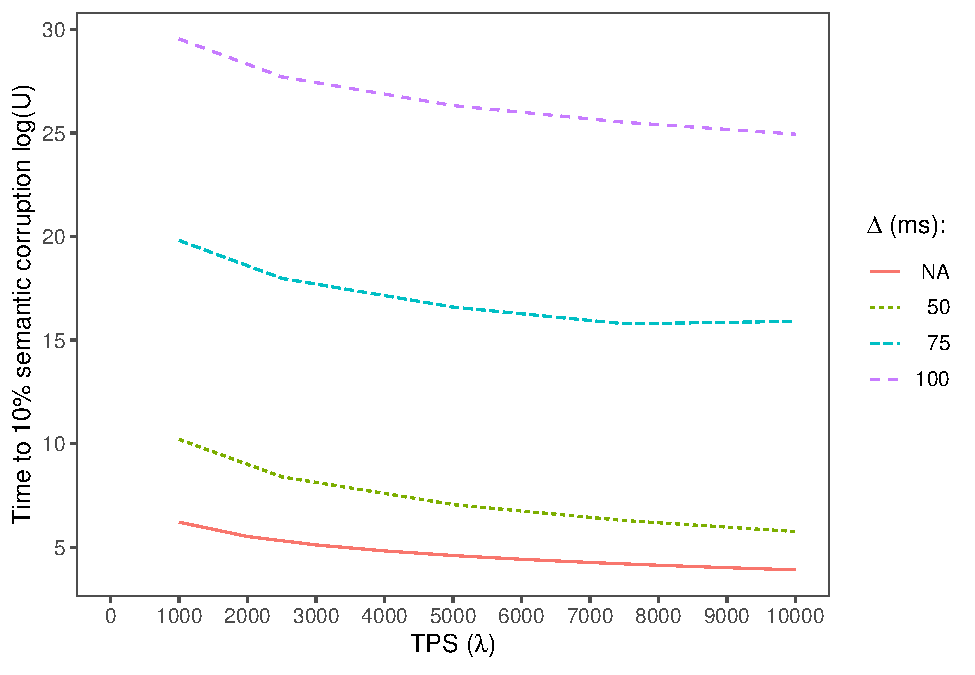
\includegraphics[width=\linewidth]{./figures/delta}
  \caption{Time, $\log(U)$, until operational corruption ($\gamma = 0.1$) for $\Delta = 50, 75, 100ms$.}
  \Description{Graph representation.}
  \label{time-to-corruption-results}
\end{figure}

The abort rates for $\Delta = 50, 75, 100ms$ are given in Figure \ref{aborts-results} for the most popular edge type, $N=10^4$. The simulation was ran for 10 seconds for a range of transaction arrival rates, $\lambda = (1000, ..., 10000)$. For $\Delta = 50$ the abort rate varies between $1-5\%$, this increases to between $1-7\%$ and $1-9\%$ for $\Delta = 75$ and $\Delta = 100$ respectively.

\begin{figure}[h]
  \centering
  % 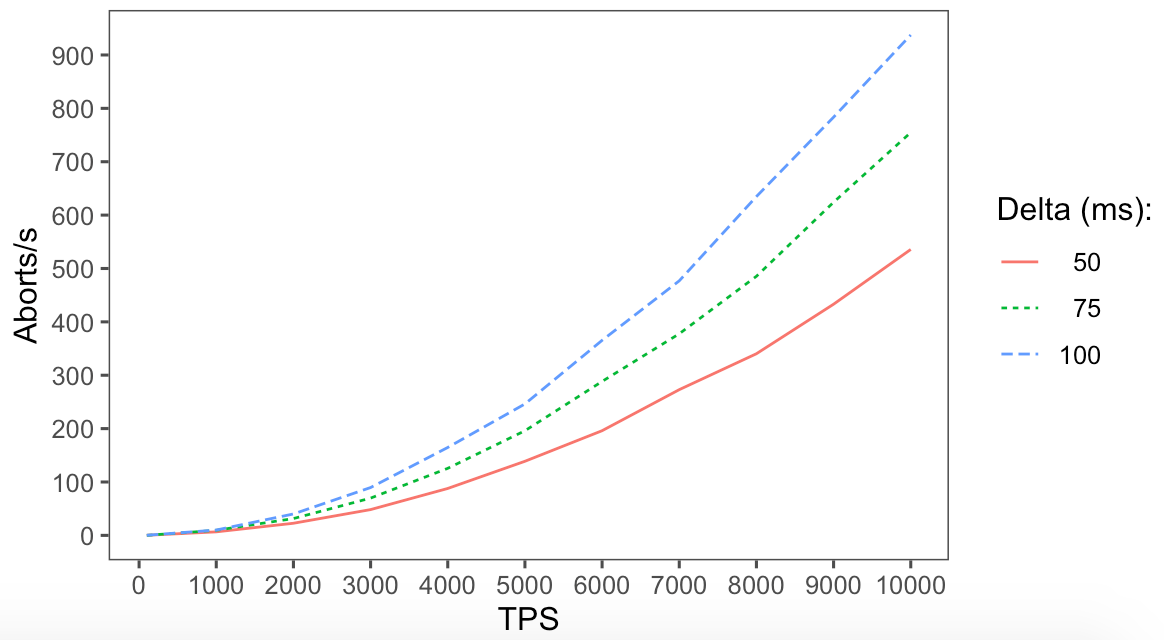
\includegraphics[width=\linewidth]{./figures/aborts_50_75_100}
 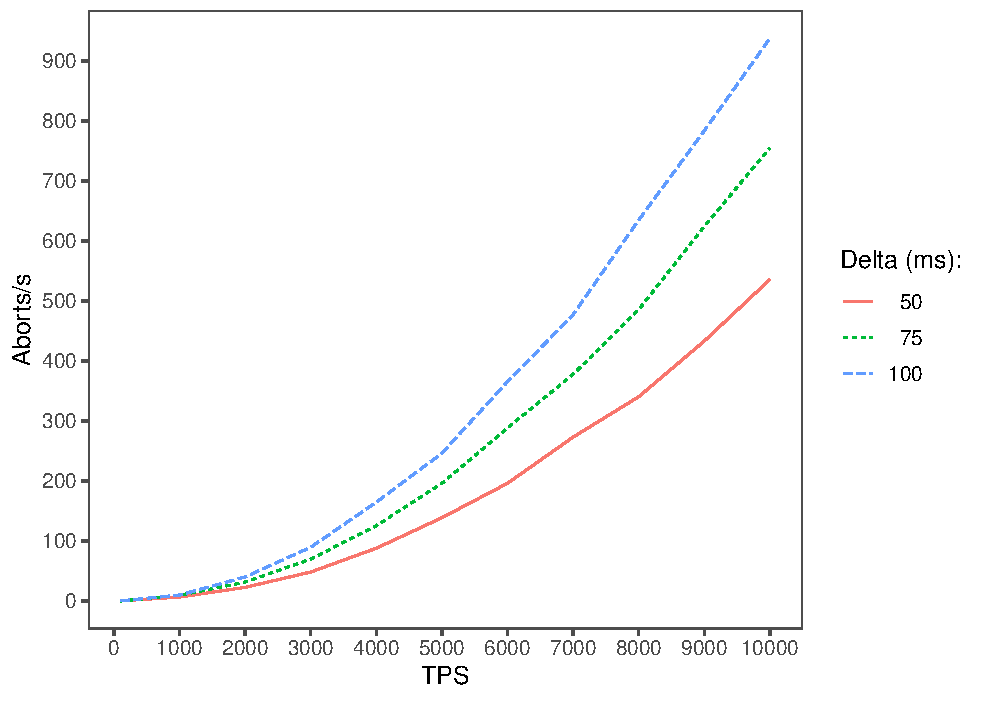
\includegraphics[width=\linewidth]{./figures/aborts}
  \caption{Aborts per seconds for $\Delta = 50, 75, 100ms$.}
  \Description{Graph representation.}
  \label{aborts-results}
\end{figure}


\section{Conclusions}

Database concurrency control has been a long researched area, however to the best of our knowledge this is first attempt at a developing protocol specific for distributed graph databases. We presented a lightweight protocol for providing reciprocal consistency and mitigating the problem of high contention in a distributed graph database. The \tDelta protocol leverages the fact writes to distributed edges always consists of two sequential writes to entries in the adjacency lists of vertices the edge connects. The protocol provides guarantees weaker than Read Uncommitted isolation (the weakest ANSI isolation level). However, such a mechanism is believed to be valuable in practice, given the popularity of BASE distributed graph databases and the rate at which corruption can spread if left unchecked. Simulations indicate the protocol rules out corruption resulting from half-corrupted distributed edges in realistic database lifetime, with the abort rate being in a reasonable range. For future work, we intend on implementing the protocol to assess the validity of the simulations and measure performance against a BASE distributed graph database operating without any concurrency control. Moreover, we plan on investigating the suitability of higher isolation levels in a distributed graph database, \textbf{Read Atomic} isolation \cite{Bailis2014} seems particularly well suited.


% \appendix
% \section{Appendix}

% Figure \ref{corruption-again} presents an interleaving when a distributed edge can become half-corrupted under the \tDelta protocol.

% Transaction $T_x$ arrives at $S_i$ at time $t_x$ (let $t=0$) and writes tentatively, with the message delay between servers for $T_x$ to write the edge at $S_j$ being $M_x$. Transaction $T_y$ arrives at $S_j$ at time $t_y$ ($t_y > t_x$) and writes the distributed edge, $T_y$ then takes time $M_y$ to write the edge at $S_i$. If $T_x$ arrives at $S_j$ after $t_y + \Delta$ and $T_y$ arrives at $S_i$ after $t_x + \Delta$ the edge can become half-corrupted. Letting $t_x = 0 $, the probability that $T_x$ and $T_y$ conflict can be formulated as: $$ P \left[ ( T_x >  \Delta + X) \cap (T_y > \Delta-X) \right]$$.

% The arrival times of $T_x,T_y$ are assumed exponentially distributed , $T \sim \exp (\rho)$. Where, $ \rho  = \frac{\lambda P_i}{2N_i}$, the probability a given operation accesses the incorrect record of a half-corrupted edge of type $i$. The transmission times between servers $M_1, M_2 \sim \exp (\delta)$ and are \emph{iid}.

% % Therefore,  $$ g(y) = \delta e^{-\delta y} $$

% Therefore,
% \begin{dmath*}
%   q^{new}_{i} =  {P \left[ ( T_1 >  d + X) \cap (T_2 > d-X)  \right]} \\
%   =  \int_{0}^{d}  \frac{\lambda P_i}{2 N_i} e^{-\frac{\lambda P_i}{2 N_i} x} e^{-\delta (d+x)} e^{-\delta (d-x)} dx + \int_{d}^{\infty} \frac{\lambda P_i}{2 N_i} e^{-\frac{\lambda P_i}{2 N_i} x} e^{-\delta (d+x)} dx  \\
%   =  e^{-2 d \delta} - \left( \frac{\delta}{\frac{\lambda P_i}{2 N_i} + \delta} \right) e^{-(\frac{\lambda P_i}{2 N_i}+ 2\delta)d} \\
% \end{dmath*}

% To choose to bound $\Delta$ consider the probability of the message delay exceeding  $\Delta$.
% \begin{align*}
%   P \left[ M > \Delta \right] & = 1 - e^{- \delta \Delta} \\
%   1 - e^{- \delta \Delta} & = 1 - \epsilon \\
%   e^{- \delta d} & = \epsilon  \\
%   \Delta & = - \frac{\ln(\epsilon)}{\delta}
% \end{align*}

% Substituting $\Delta$ into the above equation yields the conflict probability for a given $\epsilon$. For example, $ e = 0.001$ gives a $0.001$ \% probability the message delay exceeds $\Delta$, for this  $\Delta = 0.035s$
% \begin{align}
%   e^{- \lambda d} =  e^{-\delta d \frac{\lambda}{\delta}} = \epsilon^{\frac{\lambda}{\delta}} \label{eqn7}
% \end{align}
% Therefore, from (\ref{eqn5} and  (\ref{eqn7}),
% \begin{align}
%   & = \epsilon^2 - \frac{\delta}{\frac{\lambda P_i}{2 N_i} + \delta} e^{-\frac{\lambda P_i}{2 N_i} d} \epsilon^2 \\
%   & = \epsilon^2 \left[1 -\frac{\delta}{\frac{\lambda P_i}{2 N_i} + \delta} e^{-\frac{\lambda P_i}{2 N_i} d} \right]
% \end{align}


%Where, $ E \left[ T_1 \right] = E \left[ T_2\right] = \frac{1}{\delta}$.
%Therefore, $$ f(x) =\frac{\lambda P_i}{2N_i} e^{-\frac{\lambda P_i}{2N_i} x} $$

%  =   \int_{0}^{d}  \frac{\lambda P_i}{2 N_i} e^{-\frac{\lambda P_i}{2 N_i} x} e^{-\delta 2 d} dx +  \int_{d}^{\infty} \frac{\lambda P_i}{2 N_i} e^{-\delta d} e^{-(\frac{\lambda P_i}{2 N_i} + \delta)x}  dx  \\
%         =   e^{-2 d \delta} \left[1 - e^{-\frac{\lambda P_i}{2 N_i} d} \right] + \frac{\frac{\lambda P_i}{2 N_i} e^{-\delta d}}{\frac{\lambda P_i}{2 N_i} + \delta} e^{-(\frac{\lambda P_i}{2 N_i} + \delta)d} \\

\bibliographystyle{ACM-Reference-Format}
\bibliography{papoc}

\end{document}
\endinput
